\documentclass{article}

\usepackage[latin1]{inputenc}
\usepackage{color}
\usepackage{listings}
\usepackage[english]{babel}
\usepackage{graphicx}
\usepackage{indentfirst}
\usepackage{amsmath,amsfonts,graphicx}

%\usepackage{fontspec}
%\usepackage[utf8]{inputenc}
%\setmainfont{Futura}[ItalicFont={Futura Italic}]

\definecolor{colKeys}{rgb}{0,0,1}
\definecolor{colIdentifier}{rgb}{0,0,0}
\definecolor{colComments}{rgb}{0,0.5,1}
\definecolor{colString}{rgb}{0.6,0.1,0.1}


\parskip 5pt plus 2pt minus 2pt
\textwidth=17.5cm
\oddsidemargin=-0.5cm
\evensidemargin=-0.5cm
\topmargin=-0.25cm
\headheight=0cm
\headsep=1cm
\textheight=23cm
\parindent=0cm

\begin{document}
\thispagestyle{empty}
\begin{center}
\fbox{\large\bf Frequency Response Techniques in Control Systems}
\end{center}
\bigskip

Let's assume $u(t)$, $y(t)$, and $G(t)$ represents the input, output,
and transfer function representation of an input-output continuous time
system.

In order to characterize frequency response of a dynamical system,
the test signal is 
%
\begin{align*}
 u(t) = e^{j \omega t}
\end{align*}
%
which is an artificial complex periodic signal with a 
frequency of $\omega$. The Laplace transform of $u(t)$ takes the
form
%
\begin{align*}
 U(s) = \mathcal{L} \lbrace e^{j \omega t} \rbrace = \frac{1}{s - j \omega}
\end{align*}
%
Response of the system in s-domain is given by
%
%
\begin{align*}
 Y(s) = G(s) U(s) = G(s) \frac{1}{s - j \omega}
\end{align*}
%
Assuming that $G(s)$ is a rational transfer function
we can perform a partial fraction expansion
%
\begin{align*}
     Y(s) &= \frac{a}{s -  j \omega} + \left[ \mathrm{terms \ due \
  to \ the \ poles \ of} \  G(s) \right] 
\\
a &= \lim_{s \to j \omega} \left[ (s - j \omega) Y(s)
  \right]  = G(j \omega)
\\
Y(s) &=  \frac{G(j \omega)}{s -  j \omega} + \left[ \mathrm{terms \ due \
  to \ the \ poles \ of} \  G(s) \right]  
\end{align*}
%
Taking the inverse Laplace transform yields
%
\begin{align*}
  y(t) = G(j \omega) e^{j \omega t} + \mathcal{L}^{-1} \left[ \mathrm{terms \ due \
  to \ the \ poles \ of} \  G(s) \right]  
\end{align*}
%
If we assume that the system is ``stable'' or system is a part of
closed loop system and closed loop behavior is stable then
at steady state we have
%
\begin{align*}
y_{ss}(t) &= G(j \omega) e^{j \omega t} \\
&= | G(j \omega) | e^{i \omega t + \angle [ G(j \omega) ] }
\\
&= M e^{i \omega t + \theta}
\end{align*}
%
In other words complex periodic signal is scaled and phase shifted
based on the following operators
%
\begin{align*}
M &= | G(j \omega) | \\
\theta &= \angle G(j \omega)
\end{align*}
%
It is very easy to show that for a general real time domain signal
$u(t) = \sin (\omega t + \phi)$, the output $y(t)$ at steady state 
is computed via
%
\begin{align*}
  y_{ss}(t) = M \sin(\omega t + \phi + \theta)
\end{align*}
%

\newpage

\section*{2. Plotting Frequency Response: Polar Plot}

We can consider the frequency response function $G(j \omega)$
as a mapping from positive $j \omega$ axis to a curve in 
the complex plane. In polar plot, we draw the frequency response
function starting from $\omega = 0$ (or $\omega \to 0^+$) to $\omega
\to \infty$.

Let's draw the polar plots of 
%
\begin{align*}
 G_1(s) &= s
 \quad , \quad
 G_2(s) = \frac{1}{s}
 \quad , \quad
 G_3(s) = s + 2
\\
 G_4(s) &= 2 + \frac{1}{s}
\quad , \quad
 G_5(s) = 2 + s +  \frac{1}{s}
\end{align*}

\vspace{6 pt}

  \begin{minipage}[h]{1\linewidth}
    \begin{center}
      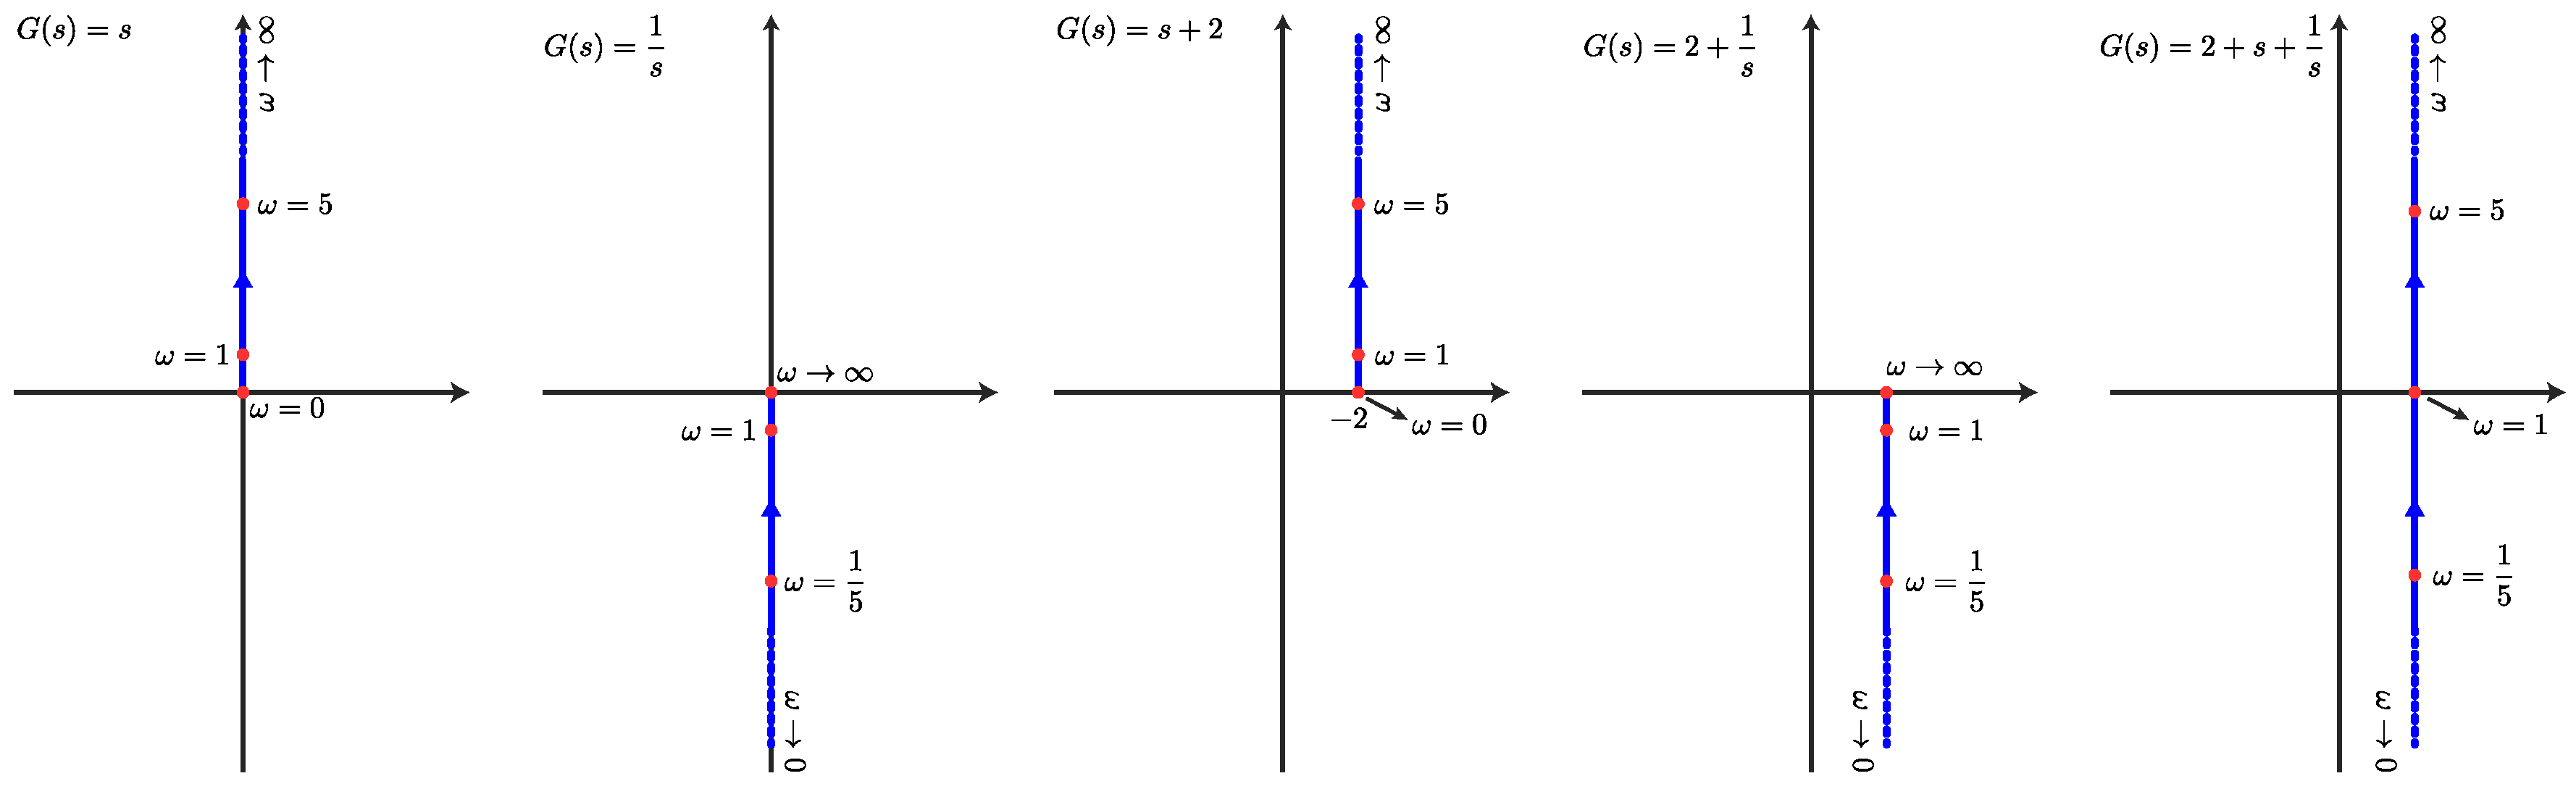
\includegraphics[width=0.99\textwidth]{polar}
    \end{center}
  \end{minipage}

\vspace{6 pt}

\textbf{Ex:} Draw the polar plots of 
%
\begin{align*}
 G_1(s) &= \frac{1}{s+1}
 \quad , \quad
 G_2(s) = \frac{s}{s+1}
\end{align*}

Let's analyze $G_1(j \omega)$ for $\omega \in [0 , \infty)$

\begin{align*}
 G_1(j \omega) &= \frac{1}{j \omega +1} = \frac{1 - j \omega}{\omega^2 +1} 
= \frac{1}{\omega^2 +1} - \frac{\omega}{\omega^2 +1} j
\\
| G_1(j \omega) | &= \frac{1}{ \sqrt{1 + \omega^2} }
\\
\angle [ G_1(j \omega) ] &= \arctan (-\omega) 
\end{align*}

Now let's analyze $G_2(j \omega)$ for $\omega \in [0 , \infty)$

\begin{align*}
 G_2(j \omega) &= \frac{j \omega}{j \omega +1} = \frac{j \omega + \omega^2}{\omega^2 +1} 
= \frac{\omega^2}{\omega^2 +1} + \frac{\omega}{\omega^2 +1} j
\\
| G_2(j \omega) | &= \sqrt{ \frac{ \omega^2 }{ 1 + \omega^2 } }
\\
\angle [ G_2(j \omega) ] &= \arctan (1 / \omega) 
\end{align*}

Polar plots of $G_1(s)$ and $G_2(s)$ are illustrated below. 

\vspace{6 pt}

  \begin{minipage}[h]{1\linewidth}
    \begin{center}
      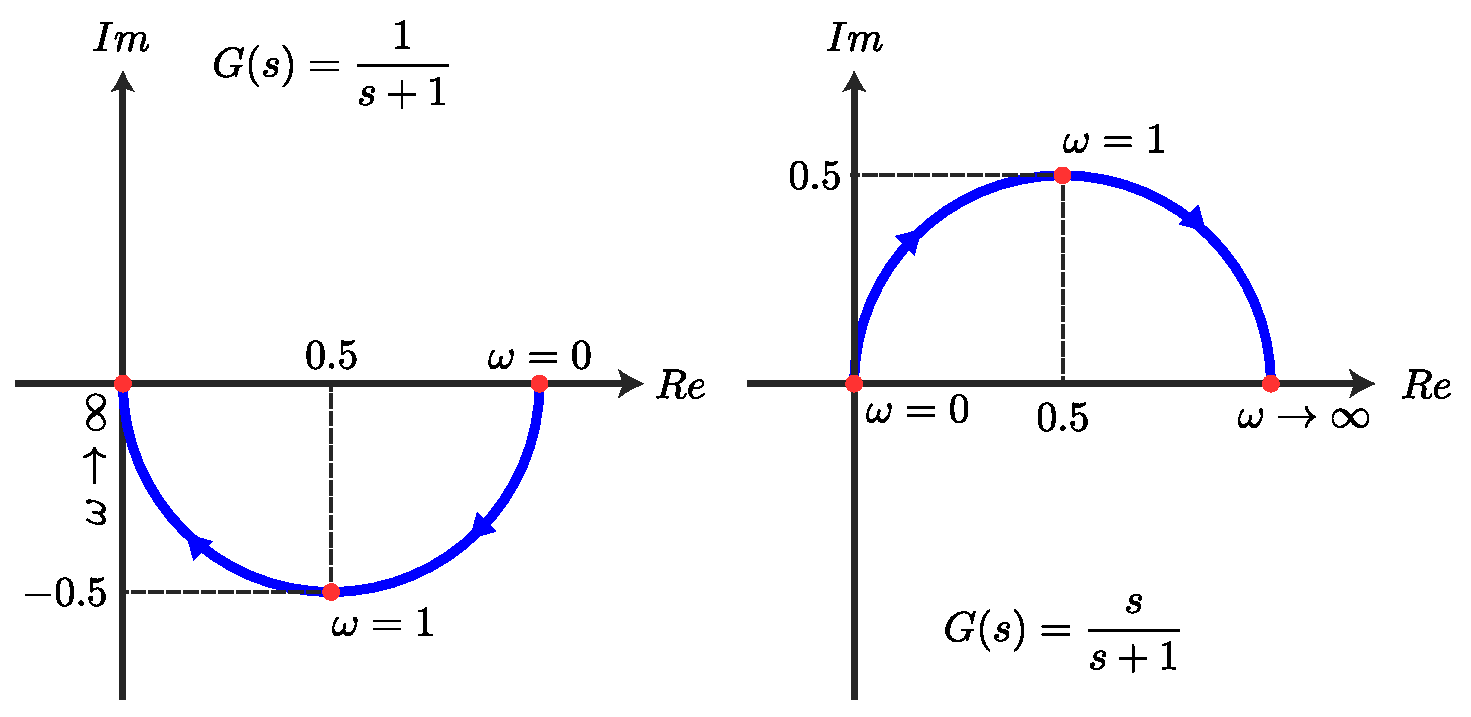
\includegraphics[width=0.8\textwidth]{polar2}
    \end{center}
  \end{minipage}

\vspace{6 pt}

\textbf{Ex:} Draw the polar plot of  $G(s) = \frac{1}{(s+1)^2}$
%
\begin{align*}
  G(j \omega ) &= \frac{1}{ (j \omega + 1)^2 } = \frac{ (-j \omega + 1)^2 }{( \omega^2 +1 )^2 }
\\
&= \left[ \left( 1 - \omega^2 \right) + j ( - 2 \omega) \right] \frac{1}{( \omega^2 +1 )^2 }
\end{align*}
%
Some important points and associated features on the polar plot can be computed as
\begin{align*}
  \omega &\to 0 \ \Rightarrow G(j \omega) = 1
\\
 \omega &\to 1 \ \Rightarrow G(j \omega) = -0.5 j 
\\
 \omega &\to  \infty \ \Rightarrow | G(j \omega) | \to 0 \quad \& \quad \angle  [ G(j \omega) ] \to -\pi
\end{align*}

Resultant polar plot is illustrated below

\vspace{6 pt}

  \begin{minipage}[h]{1\linewidth}
    \begin{center}
      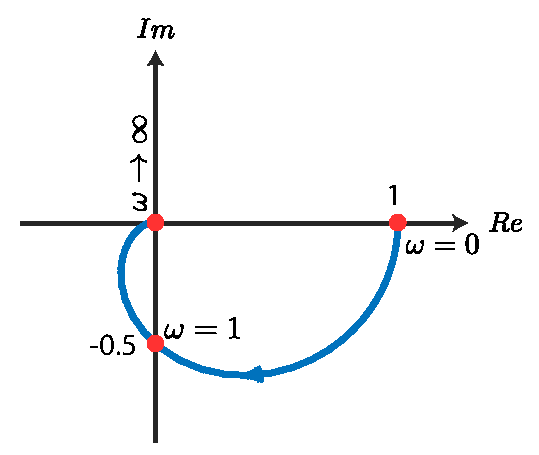
\includegraphics[width=0.45\textwidth]{polar4}
    \end{center}
  \end{minipage}

\vspace{6 pt}

\textbf{Ex:} Draw the polar plot of  $G(s) = \frac{1}{(s+1)^3}$
%
\begin{align*}
  G(j \omega ) &= \frac{1}{ (j \omega + 1)^3 } = \frac{ (-j \omega + 1)^3 }{( \omega^2 +1 )^3 }
\\
&= \left[ \left( 1 - 3 \omega^2 \right) + j (\omega^3 - 3 \omega) \right] \frac{1}{( \omega^2 +1 )^3 }
\end{align*}
%
Some important points and associated features on the polar plot can be computed as
\begin{align*}
  \omega &\to 0 \ \Rightarrow G(j \omega) = 1
\\
 \omega &\to \sqrt{1/3} \ \Rightarrow G(j \omega) = -0.65 j 
\\
 \omega &\to \sqrt{3} \ \Rightarrow G(j \omega) = -1/4 
\\
 \omega &\to  \infty \ \Rightarrow | G(j \omega) | \to 0 \quad \& \quad \angle  [ G(j \omega) ] \to \pi/2
\end{align*}

Resultant polar plot is illustrated below

\vspace{6 pt}

  \begin{minipage}[h]{1\linewidth}
    \begin{center}
      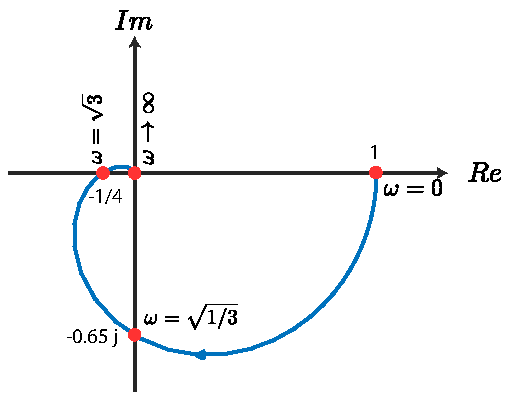
\includegraphics[width=0.5\textwidth]{polar5}
    \end{center}
  \end{minipage}

\vspace{6 pt}

\section*{2. Nyquist Contour \& Nyquist Plot}

Nyquist plot is another tool that we use to to investigate 
the stability and robustness of a feedback system. The technique 
utilizes the frequency response characteristics of a system.

\textbf{Definition:} A contour $\Gamma_s$ is a closed path with a direction
in a complex plane. 

\textbf{Remark:} A continuous function $F(s)$ maps a contour
$\Gamma_s$ in $s-$plane to another contour $\Gamma_{F(s)}$
in $F(s)$ plane. The figure below illustrates a clock-wise contour 
$\Gamma_s$ and its map $\Gamma_{F(s)}$ which is also clock-wise
in this example. 

\vspace{6 pt}

  \begin{minipage}[h]{1\linewidth}
    \begin{center}
      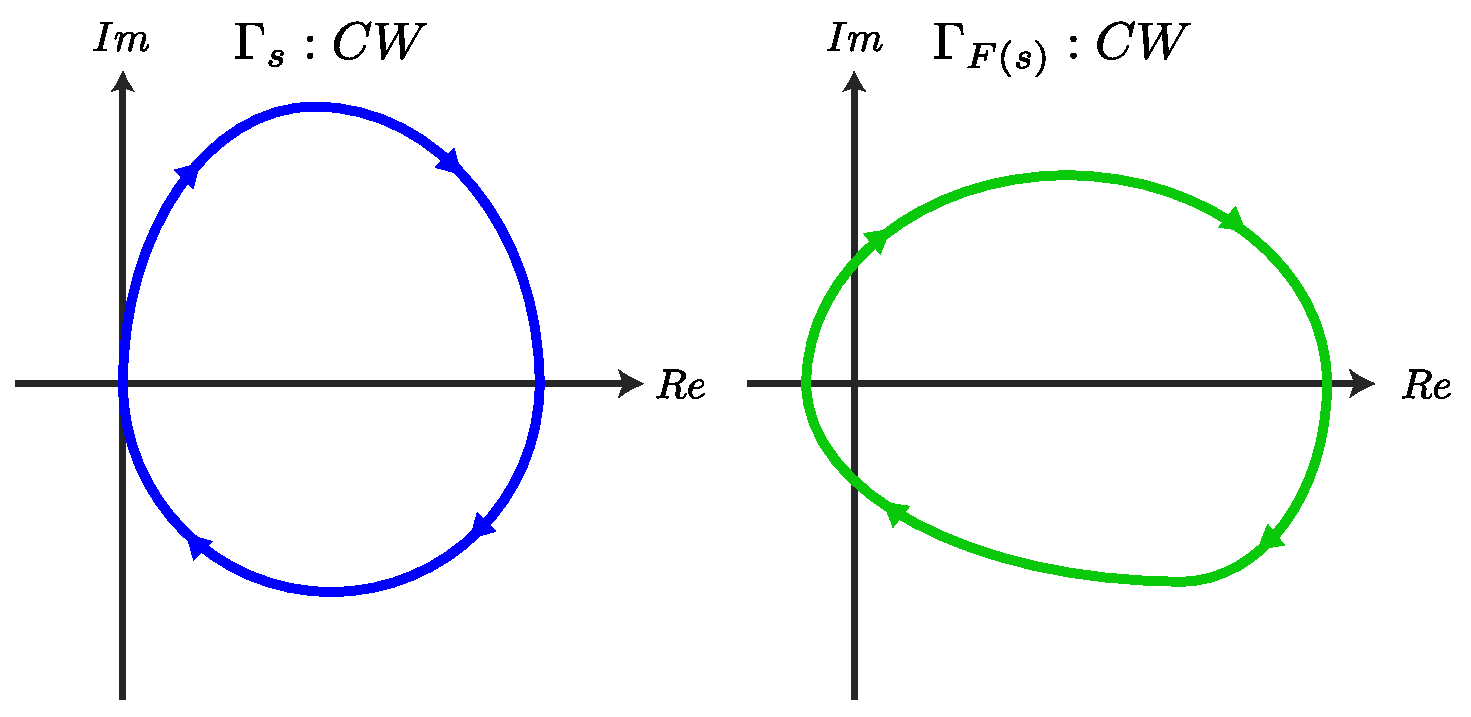
\includegraphics[width=0.75\textwidth]{cmap}
    \end{center}
  \end{minipage}
  
\vspace{6 pt}

Let's consider an LTI transfer function $G(s) = \frac{N(s)}{D(s)}$ that 
has no zeros or poles on the imaginary axis. Nyquist contour/path, 
$\Gamma_s$, is defined in a way that it covers the
whole open-right half plane. As illustrated in the Figure below, 
Nyquist contour is technically a half-circle for which the radius, $R
\to \infty$. After that, one can draw the Nyquist plot, which is the
mapped contour $\Gamma_{G(s)}$. Figure below illustrates a Nyquist
contour and associated Nyquist plot. 

\vspace{6 pt}

  \begin{minipage}[h]{1\linewidth}
    \begin{center}
      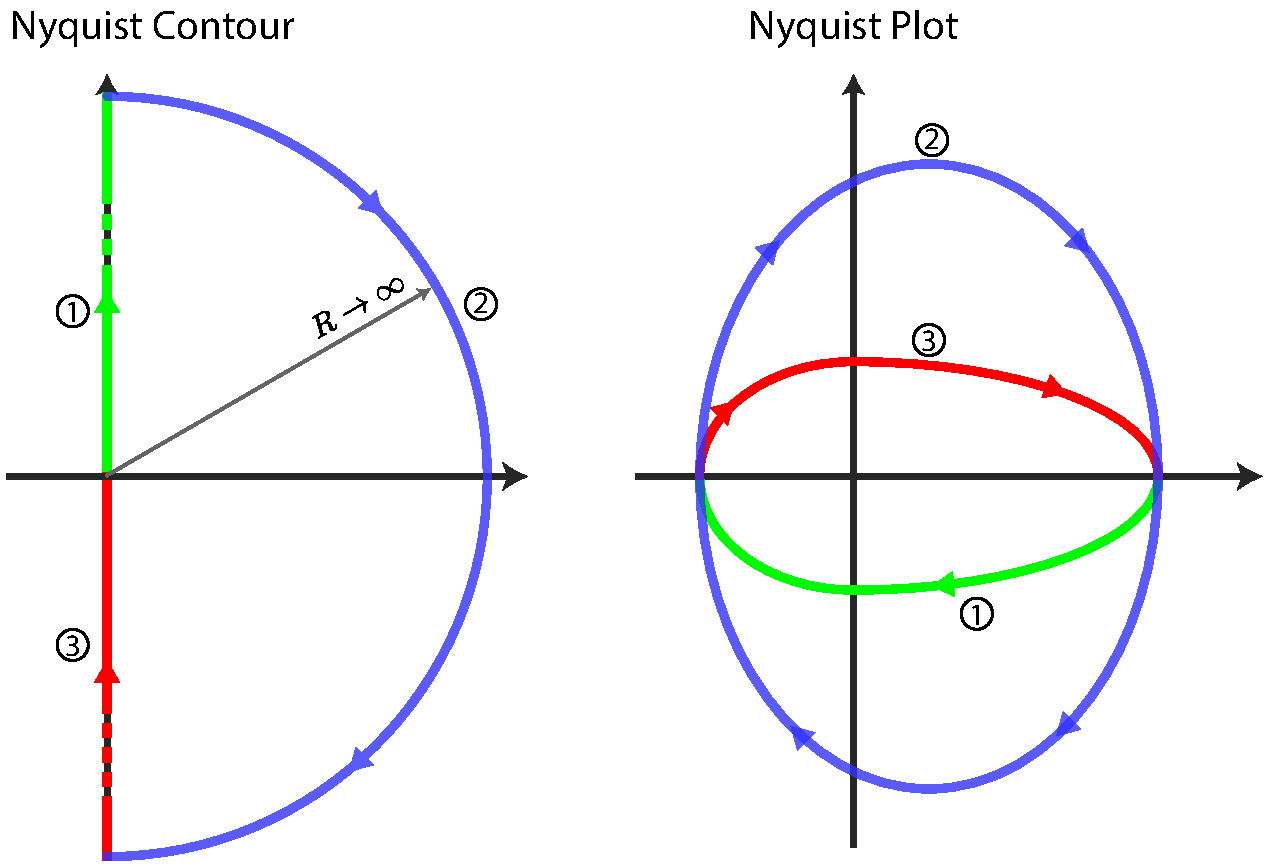
\includegraphics[width=0.65\textwidth]{nyq}
    \end{center}
  \end{minipage}

\vspace{12 pt}

\textbf{Ex:} Let's draw the Nyquist plot of $G(s) = \frac{1}{s+1}$ 

\textbf{Solution:}  Based on the Nyquist contour we have three major
paths. Now let's analyze the Nyquist paths
%
\begin{enumerate}
  \item This part corresponds to the polar plot that we covered in the previously, We already 
  plotted $G(j \omega)$, where $\omega : 0 \to \infty$. 
%
  \item This is the mapping of the infinite radius circular path on
    Nyquist contour. In this case if we write $s$ in polar form, we get 
   $s = R e^{j \theta}$ where $\theta : \pi/2 \to -\pi/2$.  Then 
   we can derive that  
   \begin{align*}
     & G \left( R e^{j \theta} \right)  \approx \frac{1}{R e^{j
       \theta}} = \frac{e^{j (-\theta)}}{R}
       \\
    &\Rightarrow | G \left( R e^{j \theta} \right) | \approx 0
   \end{align*}
   %
   \item Last path (mapping of negative imaginary axis) is simply 
    the conjugate of polar plot with reverse direction. 
\end{enumerate}

If we follow the procedure, we obtain the following Nyquist plot. 

\vspace{6 pt}

  \begin{minipage}[h]{1\linewidth}
    \begin{center}
      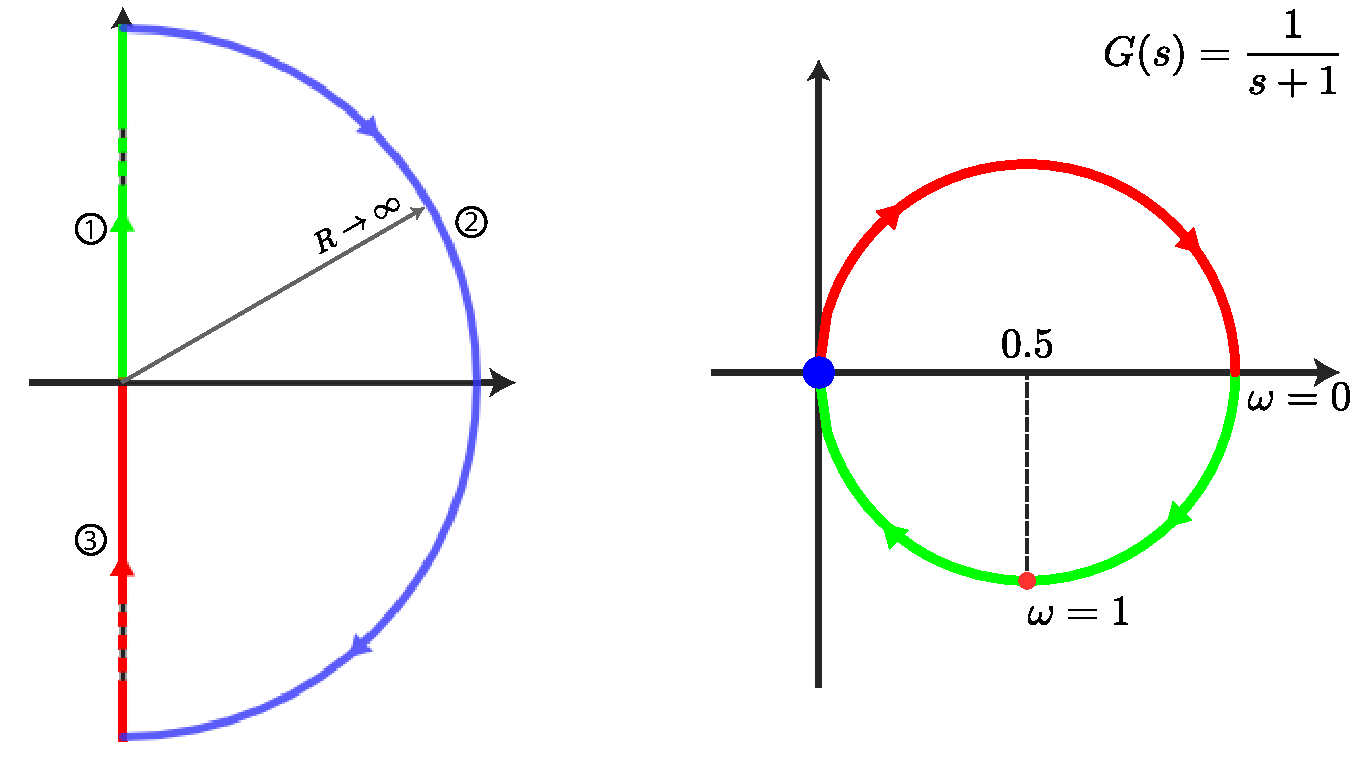
\includegraphics[width=0.75\textwidth]{ex2}
    \end{center}
  \end{minipage}

\vspace{12 pt}

\textbf{Ex:} Let's draw the Nyquist plot of 
$G(s) = \frac{1}{(s+1)^2}$ 

\textbf{Solution:} Let's analyze the Nyquist paths
%
\begin{enumerate}
  \item Mapping of first path corresponds to the polar plot that we covered in the previously. We plot $G(j \omega)$, where $\omega : 0 \to
    \infty$. 
%
  \item This is the infinite radius circular path. In this case if we write $s$ in polar form, we get 
   $s = R e^{j \theta}$ where $\theta : \pi/2 \to -\pi/2$.  Then 
   we can derive that  
   \begin{align*}
     & G \left( R e^{j \theta} \right) = \approx \frac{1}{R^2 e^{j
       2 \theta}} = \frac{e^{j (-2 \theta)}}{R^2}
       \\
    &\Rightarrow | G \left( R e^{j \theta} \right) | \approx 0
   \end{align*}
   %
   \item Last path (mapping of negative imaginaty axis) is again
   the conjugate of polar plot with reverse direction. 
\end{enumerate}

If we follow the procedure, we obtain the following Nyquist plot. 

\vspace{6 pt}

  \begin{minipage}[h]{1\linewidth}
    \begin{center}
      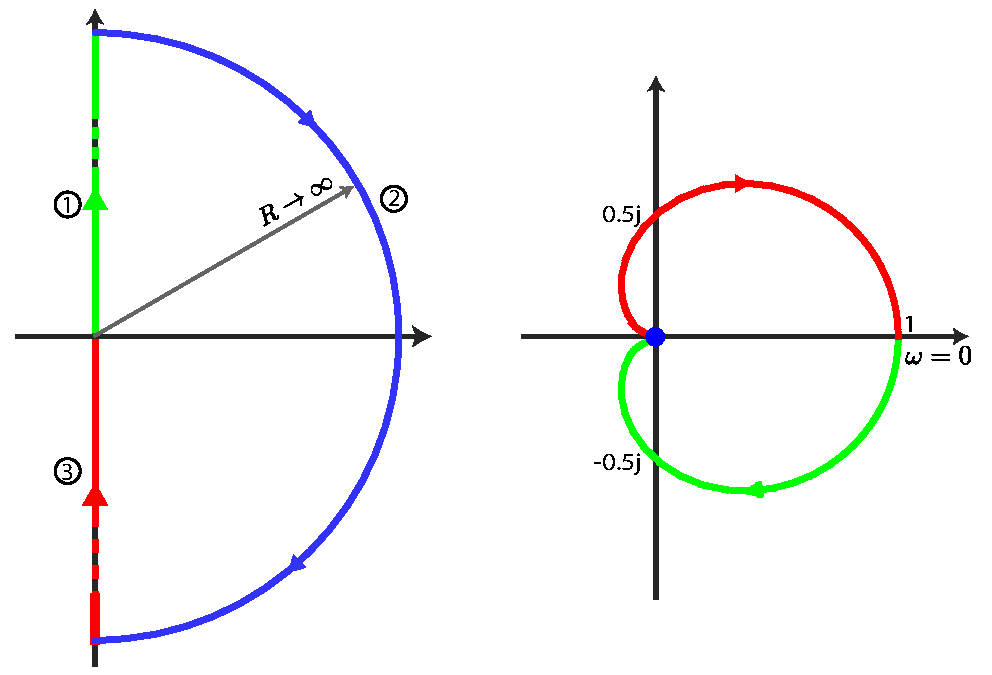
\includegraphics[width=0.75\textwidth]{ex3}
    \end{center}
  \end{minipage}

\vspace{12 pt}

\textbf{Ex:} Draw the Nyquist plot of $G(s) =
\frac{1}{(s+1)^3}$ 

\textbf{Solution:} Firs let's analyze the Nyquist paths
%
\begin{enumerate}

  \item This is the polar plot that we have covered in the previous
    lecture. We plotted $G(j \omega)$, where $\omega : 0 \to
    \infty$. 
    % 
  \item This is the mapping of the infinite radius circular path on
    Nyquist contour. In this case if we write $s$ in polar form, we
    get $s = R e^{j \theta}$ and $\theta : \pi/2 \to -\pi/2$.  Then 
   we can derive that  
   \begin{align*}
     & G \left( R e^{j \theta} \right) \approx \frac{1}{R^3 e^{j
       3 \theta}} = \frac{e^{j (-3 \theta)}}{R^3}
       \\
    &\Rightarrow | G \left( R e^{j \theta} \right) | \approx 0
   \end{align*}
   %
   \item Last path (mapping of negative imaginaty axis) is again
   the conjugate of polar plot with reverse direction. 
\end{enumerate}

If we follow the procedure, we obtain the following Nyquist plot. 

\vspace{6 pt}

  \begin{minipage}[h]{1\linewidth}
    \begin{center}
      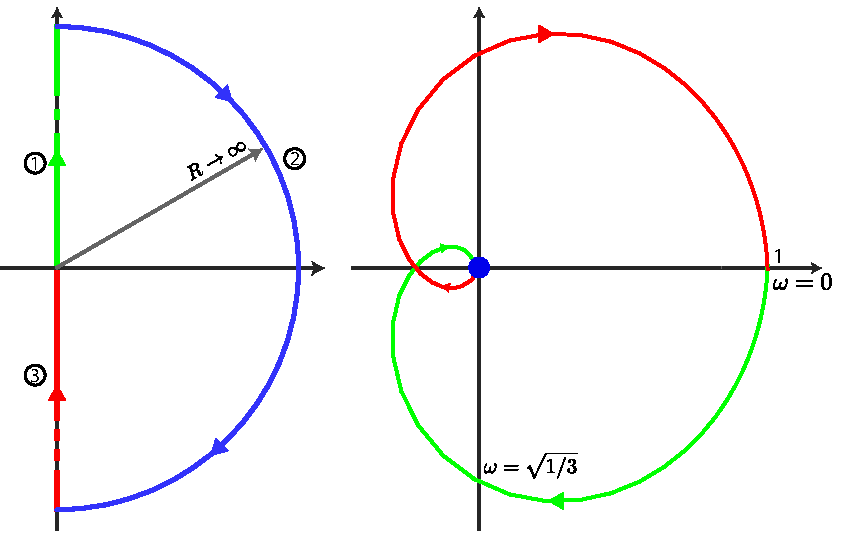
\includegraphics[width=0.75\textwidth]{ex4}
    \end{center}
  \end{minipage}

 
\end{document}
